% compter-1-10.tex
% Author: Sébastien Combéfis
% Version: June 13, 2016

\documentclass[a4paper,11pt,final]{article}

% Packages
\usepackage[utf8x]{inputenc}
\usepackage[T1]{fontenc}
\usepackage[french]{babel}
\usepackage{lmodern}

\usepackage{graphicx}
\usepackage{tikz,pgf}
\usepackage{array}
\usepackage{amssymb}
\usepackage{watermark}
\usepackage{xeCJK}
\usepackage{hyperref}
\usepackage{microtype}

% Page dimensions
\setlength\textheight{25.5cm}
\setlength\textwidth{17.5cm}
\setlength\oddsidemargin{-0.5cm}
\setlength\topmargin{-15mm}
\setlength\headheight{0mm}
\setlength\parindent{0.0cm}
\setlength\parskip{0.5cm}

% Style and fonts
\pagestyle{empty}
\urlstyle{sf}
\setmainfont{Cambria}
\setCJKmainfont{ipaexm.ttf}

% New colors
\definecolor{titleblue}{rgb}{0,0.2,0.4}
\definecolor{numberred}{rgb}{0.5,0,0}
\definecolor{sectionblue}{rgb}{0.1,0.3,0.7}
\definecolor{lightlightgray}{gray}{0.9}

% New commands
\renewcommand{\arraystretch}{1.3}
\newcommand{\trig}{\color{sectionblue}$\blacktriangleright$}
\newcommand{\sectit}[1]{\bigskip\hspace{-5mm}{\color{sectionblue}$\blacksquare$~~\Large\bfseries #1}}
\newcommand{\romaji}[1]{{\footnotesize[#1]}}

\begin{document}
	\rightwatermark{
		\begin{tikzpicture}[overlay]
			\draw[draw=none,fill=numberred] (17,-28.7) rectangle (18,-27.2);
			\node at (17.5,-27.8) {\color{white}\thepage};
			\node[anchor=west] at (-1.5,-28) {\raisebox{-0.5mm}{
\includegraphics[width=2cm]{images/by-nc-nd.pdf}}~~\small poly.glot, 2016.};
		\end{tikzpicture}
	}

% = = = = = = = = = = = = = = = = = = = = = = = = = = = = = = = = = = = = = = = = = = = = = = = = = = = =
% Compter de 1 à 10
% = = = = = = = = = = = = = = = = = = = = = = = = = = = = = = = = = = = = = = = = = = = = = = = = = = = =
\begin{tikzpicture}[overlay]
	\draw[draw=none,fill=titleblue] (4,-1) rectangle (19,1.5);
	\node[anchor=east] at (18,0.2) {\color{white}\Huge\sl Compter de 1 à 10};
	% https://openclipart.org/detail/168838/seven-segment-display-gray-7
	\node[anchor=south east] at (2.5,-1.15) {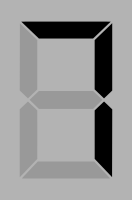
\includegraphics[width=1.5cm]{images/Seven-segment-display-gray-7-200px.png}};
\end{tikzpicture}\vspace{15mm}
	
% - - - - - - - - - - - - - - - - - - - - - - - - - - - - - - - - - - - - - - - - - - - - - - - - - - - -

On peut écrire les nombres avec la notation arabe (1, 2, 3) ou la chinoise (一, 二, 三). La première notation est plus souvent utilisée lorsqu'on écrit horizontalement et la seconde lorsqu'on écrit verticalement. Dans certain cas, pour des documents officiels notamment, on utilisera d'office la notation chinoise. Concernant la lecture, lorsqu'il s'agit de compter (nombre cardinal), on utilise généralement la prononciation \textit{on}'.

% - - - - - - - - - - - - - - - - - - - - - - - - - - - - - - - - - - - - - - - - - - - - - - - - - - - -

\sectit{De 1 à 10}
	
\hspace{5mm}\begin{tabular}{|p{1.5cm}p{1.5cm}p{3cm}p{3cm}}
	\multicolumn{1}{l}{}&& \it\small Lecture préférée & \it\small Lecture alternative \\
	1		& 一			& いち \romaji{ichi} \\
	2		& 二			& に	 \romaji{ni}		& じ \romaji{ji} \\
	3		& 三			& さん \romaji{san} \\
	4		& 四			& よん \romaji{yon}		& し \romaji{shi} \\
	5		& 五			& ご \romaji{go} \\
	6		& 六			& ろく \romaji{roku} \\
	7		& 七			& なな \romaji{nana}		& しち \romaji{shichi} \\
	8		& 八			& はち \romaji{hachi} \\
	9		& 九			& きゅう \romaji{ky\=u}	& く \romaji{ku} \\
	10		& 十			& じゅう \romaji{j\=u}
\end{tabular}

Les chiffres 4 et 9 portent malheur en japonais, et on préfère les prononcer respectivement \romaji{yon} et \romaji{ky\=u}. En effet, la prononciation de 4 \romaji{shi} est proche de celle de la \textit{mort} (死) et celle de 9 \romaji{ku} est proche de celle de la \textit{souffrance} (苦). Les chiffres 7 et 8 portent quant à eux bonheur.

% - - - - - - - - - - - - - - - - - - - - - - - - - - - - - - - - - - - - - - - - - - - - - - - - - - - -

\sectit{Prononciation}

Comme dit précédemment, on utilise donc la prononciation \textit{on}' pour faire référence aux nombres cardinaux, sauf pour 4 \romaji{yon} et 7 \romaji{nana}. On utilisera la prononciation alternative, à savoir し \romaji{shi} et しち \romaji{shichi}, pour les noms des mois et des jours, pour certaines phrases fixes et lorsqu'on compte des objets/personnes.

Enfin, lorsqu'on dicte un numéro de téléphone, 2 et 5 sont prononcés avec une plus longue voyelle, c'est-à-dire にい \romaji{nii} et ごお \romaji{goo}.

% - - - - - - - - - - - - - - - - - - - - - - - - - - - - - - - - - - - - - - - - - - - - - - - - - - - -

\sectit{Écriture}

Pour des documents officiels légaux ou financiers, il existe, comme en chinois, des kanjis plus complexes qui empêchent la falsification (un 一 se transforme facilement en un 二, 三 ou 十, par exemple). Aujourd'hui, seules les formes complexes de 1, 2, 3 et 10 sont utilisées.

\hspace{5mm}\begin{tabular}{|l*{10}{p{1cm}}}
	\multicolumn{1}{l}{} & 1 & 2 & 3 & 10 \\
	\it\small Écriture commune & 一 & 二 & 三 & 十 \\
	\it\small Écriture complexe & 壱 & 弐 & 参 & 拾
\end{tabular}

\end{document}